\section{Implementation}
\label{s:implementation}

In this section, the implementation of the distributed file system simulator will be
outlined. Firstly, the architecture of the file system will be described and how
the distributed part of the file system was simulated. The application 
interfaces will be described which serves as the file system operations that 
are supported. The communication interfaces between the different nodes will 
also be outlined.

Additionally the details of the tracking of metadata, as well as the block 
allocation policies will be described.

\subsection{Architecture}
\label{s:architecture}

The distributed file system simulator has a similar architecture to the 
Google File System. \todo[inline]{GFS Ref.} There is a single metadata node
responsible for metadata tracking of each file, and multiple data nodes which
hold the data of each file.

\begin{figure}[H]
    \centering
    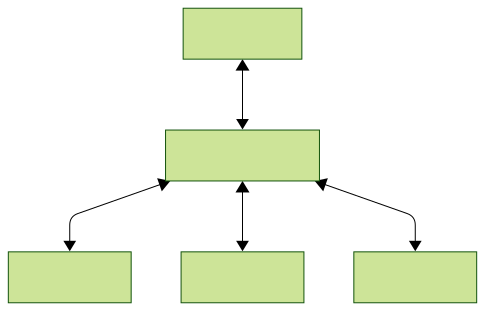
\includegraphics[width=\columnwidth]{images/architecture.png}
    \caption{Architecture Design for the Distributed File System. 
    The MetadataNode exposes the application API. The MetadataNode 
    and DataNodes communicate via the communication API.}
    \label{f:}
\end{figure}

The metadata node is connected to the various data nodes and communicates through
the communication interface. And the metadata node communicates to the workload
through the application interface.

Due to the fact that this is a distributed file system simulator, the application
all runs on the same machine. The metadata node and data nodes are simulated
as different machines by each running their own program and communicating through a
local unix socket to simulate being on different machines.

\subsection{Application API}
\label{s:applicationapi}

The application API provides an interface for interacting with the distributed 
file system simulator. It exposes functions for initializing and shutting
down the file system, creating, reading, writing, and managing file system blocks.
The API is intended to be used by client applications that need to access or
manipulate file system data while abstracting the management.

The API can be categorized into three functional groups:
\begin{itemize}
    \item \textbf{Initialization and Cleanup}: Functions to start and stop the file
    system. Involves creating the various datanodes and connecting to them.
    \item \textbf{File Management:} Functions for creating, locating, truncating, reading,
    and writing to files.
    \item \textbf{Block-level Operations:} Functions for directly reading and writing
    individual file blocks.
\end{itemize}

% DESCRIBE API

Below are the application API that describes the functions that the client or workload
can interact with.
 
\begin{lstlisting}
init(int num_dns, size_t capacity, const char *policy_name)

exit(int cleanup)

create_file(const char *filename, size_t file_size, int *fid)

find_file(const char *filename, int *fid)

truncate_file(int fid, size_t new_size)

read_file(int fid, void **buffer, size_t *file_size)

write_file(int fid, void *buffer, size_t buffer_size)

read_block(int fid, int file_index, void *buffer)

write_block(int fid, int file_index, void * buffer)
\end{lstlisting}

\subsection{MetadataNode}
\label{s:metadatanode}
The single metadatanode is responsible for keeping track of all of the file
metadata and space for the file system. It has a few data structures that are
used to keep track of this information and ensure communication between itself
and the datanodes.

\begin{figure}[H]
    \centering
    % \includegraphics[width=\columnwidth]{images/metadata_structures.png}
    \caption{.}
    \label{f:}
\end{figure}

The first few data structures relate to the internal file system information. It
keeps track of the total number of blocks available given the capacity of the
file system and keeps track of the available blocks using a \texttt{bitmap}.

The second type of data structures are related to the datanode information and tracking.
The metadanode keeps track of how many datanodes have been created for this file
system, and keeps track of connections to these datanodes. 
It also keeps a block-to-node mapping which maps the logical block of the file
system to a specific data node in the system. The metadata node also keeps track
of how full each data node is to prevent sending data to an already full data node.

The third type of data structures relate to the files metadata. It keeps track
of the number of files currently in the file system using a file structure called
\texttt{FileEntry}. Each \texttt{FileEntry} is structured with
the file name, and the number of blocks that it extends. Each file entry structure
keeps track of a file-to-block mapping, which helps us find the logical system block
given the file block (a file's block 0 might map to block 256 in the file system).

Unlike \todo[inline]{GFS}, the metadata node sits between the communication of the
workload/client and the datanodes. This is a limitation of the current design
which will be discussed in a later section. To surpass this limitation, the
current design makes it such that the metadata node and workload are simulated
to run on the same machine, meaning the workload application directly calls on
the metadata node without using commands / communication between them. This 
removes the metadata node from being the bottleneck of the application.

On initialization, the metadata node initializes the file system.
\begin{lstlisting}
metadatanode_init(int num_dns, size_t capacity, const char *policy_name)
\end{lstlisting}
The metadata node initializes the application with a specific file system size,
number of data nodes, and policy used for block allocation. This function is
responsible for creating each data node process, which is done by forking the
application and using sockets to communicate between each process. After creating
each data node, it connects to each by sending the \texttt{DN\_INIT} command to
each data node, which makes each data node initialize itself. After this function
returns, the file system is ready.

On exiting of the simulation, the metadata node can cleanup the system.
\begin{lstlisting}
metadatanode_exit(int cleanup)
\end{lstlisting}
Once this function is called, the metadata node commands each data node to shut
down. Given the parameter \texttt{cleanup}, it will order each data node to
clean up its files. The parameter can be used to inspect the imbalance and load
of each data node once the workload has finished.

The metadata node can create files with a given file size, and returns a file
id which identifies the file until closing.
\begin{lstlisting}
metadatanode_create_file(const char *filename, size_t file_size, int *fid)
\end{lstlisting}
The \texttt{fid} serves similar to an inode. 
There are various different implementations that were tested when calling this
function. Given the file size, the blocks could be allocated at this point, or
they could be allocated on write. The different implementations around when to
allocate blocks is discussed in a later section.

The metadata node is responsible for truncating a file.
\begin{lstlisting}
metadatanode_truncate_file(int fid, size_t new_size)
\end{lstlisting}
A file can be increased in size or decreased in size. On decrease, the metadata
node frees the relevant blocks based on the new size, it sends a \texttt{DN\_FREE\_BLOCK}
to each node for the block to free its memory. On increase, two things can happen,
either the blocks are allocated right away in each node, or just the metadata is 
allocated (similar to create file, blocks can be allocated on write).

\begin{lstlisting}
metadatanode_read_file(int fid, void **buffer, size_t *file_size)
\end{lstlisting}

\begin{lstlisting}
metadatanode_write_file(int fid, void *buffer, size_t buffer_size)
\end{lstlisting}

\begin{lstlisting}
metadatanode_read_block(int fid, int file_index, void *buffer)
\end{lstlisting}

\begin{lstlisting}
metadatanode_write_block(int fid, int file_index, void * buffer)
\end{lstlisting}

\subsection{Communication API}
\label{s:communicationapi}

The communication API provides an interface for the communication between the
metadatanode and the datanodes in the distributed file system. It exposes
functions for each type of node to send commands, receive commands,
and responses to the commands.

The communication is two directional but initiated by the metadata node, meaning
the metadata node sends commands, and each datanode responds.

There are six types of commands that the metadatanode can use to communicate with
the datanode \texttt{DN\_INIT}, \texttt{DN\_ALLOC\_BLOCK}, 
\texttt{DN\_FREE\_BLOCK}, \texttt{DN\_READ\_BLOCK}, \texttt{DN\_WRITE\_BLOCK}, 
\texttt{DN\_EXIT}. Each command is used alongside a buffer which sends the appropriate
information for that command. For example, \texttt{DN\_READ\_BLOCK} requires the
block index to be read.

Metadata sends commands through the following function.
\begin{lstlisting}
md_send_command(int sock_fd, DNCommand cmd, void *payload, size_t payload_size)
\end{lstlisting}
This function sends the command to the metadata node alongside the payload size (buffer
size) and then sends payloads in another request. The separation between the command
packet and payload packet was due to the fact that the command packet is quite small
and this sent faster to prepare the datanode for incomming data. The payload packet
can be quite large if we're sending multiple blocks to this data node.

The metadata receives responses through the following function.
\begin{lstlisting}
md_recv_response(int sock_fd, DNStatus *status, void **payload, size_t *payload_size)
\end{lstlisting}
If the datanode fails, the metadata node is responsible for handling that error.
In this simulator, datanode errors are only due to system errors such as out of memory
or IO errors when reading file blocks. Usually upon an error, the system shuts down.
Further considerations regarding reliability will be discussed in the further considerations
sections.

The datanode is responsible for receiving commands.
\begin{lstlisting}
dn_recv_command(int sock_fd, DNCommand *cmd, void **payload, size_t *payload_size)
\end{lstlisting}
The datanode is constantly listening for commands in the service loop, and once
a command is received, it reads the command and payload expected for that command.

The datanode sends responses to the metadata node to maintain correctness.
\begin{lstlisting}
dn_send_response(int sock_fd, DNStatus status, void *payload, size_t payload_size)
\end{lstlisting}
As mentioned previously, the simulator mostly sends success codes back to the
metadata node during normal execution.

\subsection{DataNode}
\label{s:datanode}

The data nodes are responsible for storing the contents of each logical block
of the file system. Each datanode must keep track of a few data structures.

The first involves the connection to the metadata node. As mentioned previously
a socket connection is used to communicate between the nodes. Thus each data
node keeps track of the socket to communicate with the metadata node.

The data node additionally keeps track of blocks by storing them directly on
the underlying file system. On a write, when a data node receives a logical block along
with its contents, it stores them in a file \texttt{block\_id.dat}.

The datanode implementation will be described below.

The first function of the data node application is the service loop.
\begin{lstlisting}
datanode_service_loop(int sock_fd)
\end{lstlisting}
Once the metadata node creates each data node, each data node begins in this loop.
The service loop is one in which the data node is continually listening to the
metadata node waiting for commands. Once a command is received, the specific
command is handled and the data node goes back to listening for further commands.
The command implementations are described below.

The first command that the metadata node sends after creating each data node is
\texttt{DN\_INIT}. This command fills the purpose of initializing each data node.
\begin{lstlisting}
datanode_init(int sock_fd, void *payload, size_t payload_size)
\end{lstlisting}
It initializes each data node with the node id and the capacity of this node. 
Since the simulator runs on one machine, the datanode creates a directory for 
itself where it will store the file blocks. Each data node only has access to its
own directory (identified by its node id).

The metadata node can send a command to write to a block through \texttt{DN\_WRITE\_BLOCK}.
\begin{lstlisting}
datanode_write_block(int block_index, void * buffer)
\end{lstlisting}
This function handles writing the buffer to a block with index \texttt{block\_index}.
As mentioned previously, the data node writes/overwrites the file to its directory.
Since data nodes store files of logical blocks of the file system, there are no
conflicts.

The metadata node can send a command to read a block through \texttt{DN\_READ\_BLOCK}.
\begin{lstlisting}
datanode_read_block(int block_index, void * buffer)
\end{lstlisting}
This function handles reading the file stored in the data nodes directory with the
relative block index, and write it to the buffer in preparation to send.

The metadata node can send a command to free a block through \texttt{DN\_FREE\_BLOCK}.
\begin{lstlisting}
datanode_free_block(int block_index)
\end{lstlisting}
This function handles freeing a block from teh file system. The data node finds
the file and unlinks it to free its space from the file system.

The metadata node can send a command to exit the application through \texttt{DN\_EXIT}.
\begin{lstlisting}
datanode_exit(int cleanup, int * sock_fd)
\end{lstlisting}
On exit, each data node will clean up its resources. It will free the data node 
structure and free every file that is stored in its directory.

\subsection{Policies}
\label{s:policies}

The simulator was designed to be able to handle different block allocation
policies. Initially, the focus of the simulator was to study the block
allocation strategies and how they would affect the simulator.

However due to the sequential nature of the current simulator, the policies
perform quite similarly.

Below are described the block allocation policies.

\subsubsection{Random}
Random allocation policy uses a random number to decide between the nodes.
However, blocks are not attempted to be allocated on an already full node, so
if the node is full, another pass of the random number is generated. This is
done until the number of nodes attemps has passed, then we just loop through
the nodes in order to find an available node.

\subsubsection{Sequential}
Sequential allocation policy allocates on the same node starting from node 0
until the node becomes full. Then it allocates on the next node until it becomes
full. This process repeats. Thus a file that is created, will be allocated on
the same node.

\subsubsection{Round Robin}
Round robin allocation policy allocates a block according to round robin. Round
robin initially starts with node 0 and allocates a block on each node before
allocating back on node 0.

\subsubsection{Least Loaded}
Least loaded allocation policy allocates a block on the least loaded node. This
allocation policy attempts to balance the load on each node.

\subsubsection{File Aware}
File aware allocation policy is a hybrid allocation policy which defines a
parameter \texttt{SMALL\_FILE\_THRESHOLD}. If the number of blocks to be 
allocated at the same time is lower than this threshold, the random policy is 
used, if the number of blocks to be allocated is larger, all of the blocks
are allocated on the least loaded node. This allocation policy was an attempt
to speed up the common case of small files since finding the least loaded node
requires looping through each node's metadata to find the least loaded node.

\subsection{Experiments}

\subsection{Workloads}
\label{s:workloads}

\subsection{Designs}

Various different designs where considered to investigate when blocks should
be allocated on each datanode and how to allocate the blocks. Each design is
described below.

\subsubsection{Preallocate on Create}
The first design considered was to pre-allocate all of the necessary blocks
for a file on file creation. During file creation, the file size is known since
it is a parameter. Thus the number of blocks for that file is known at this point.
At this point, the metadata node can allocate these blocks using the block 
allocation policy and send each involved data node a command to allocate a block.
Each data node will then create a file for that logical block and stored it in the
file system. 

This design was considered since at this point, the work of allocating blocks 
and creating the files is complete. And then on a write to the file, the files
would be populated without the overhead of creating the file. This design
was considered with speed in mind.

\subsubsection{Postallocate on Write}
The second design considered was to post-allocate (lazy allocate) necessary 
blocks on block/file writes. During file creation, only the metadata is modified
in the datanode and no communication to the nodes is sent. On a block write,
the metadata node will send a write command to the involved node. The data
node will then be responsible for creating this file and storing the block contents.

The design was considered to solve two considerations. The first consideration is
of space, although the common case is to write the file block by block without
blocks, there might be cases where file blocks are allocated by have no actual
data inside. With the previous design, these blocks would be allocated on the
data node, thereby reducing the space of the data node with empty blocks.

The second consideration was speed ?

\subsubsection{Batch Operations per Node}
The third design considered was batching of blocks. In the two previous designs,
operations

